\documentclass[12pt]{article}
\usepackage{graphicx}
\usepackage[german]{babel}
\usepackage{url}
\usepackage{listings}
\usepackage{color}
\usepackage{subcaption}
\usepackage{mwe}

\begin{document}

\definecolor{dkgreen}{rgb}{0,0.6,0}
\definecolor{gray}{rgb}{0.5,0.5,0.5}
\definecolor{mauve}{rgb}{0.58,0,0.82}
\definecolor{backcolour}{rgb}{0.95,0.95,0.92}
\definecolor{gray}{rgb}{0.4,0.4,0.4}
\definecolor{darkblue}{rgb}{0.0,0.0,0.6}
\definecolor{cyan}{rgb}{0.0,0.6,0.6}

\lstset{frame=tb,
  backgroundcolor=\color{backcolour},   
  aboveskip=3mm,
  belowskip=3mm,
  showstringspaces=false,
  columns=flexible,
  basicstyle={\small\ttfamily},
  numbers=none,
  numberstyle=\tiny\color{gray},
  keywordstyle=\color{blue},
  commentstyle=\color{dkgreen},
  stringstyle=\color{mauve},
  breaklines=true,
  breakatwhitespace=true,
  tabsize=3
}
\lstdefinelanguage{XML}
{
  morestring=[b],
  morestring=[s]{>}{<},
  morecomment=[s]{<?}{?>},
  stringstyle=\color{black},
  identifierstyle=\color{darkblue},
  keywordstyle=\color{cyan},
  morekeywords={xmlns,version,type}% list your attributes here
}

\begin{titlepage}
	\centering
	
\includegraphics[width=0.45\textwidth]{pictures/GestureCookLogo.png}\par\vspace{0.5cm}
	{\scshape\LARGE Kantonsschule Wohlen \par}
	\vspace{0.2cm}
	{\scshape\Large Projektunterricht\par}
	\vspace{1.5cm}
	{\huge\bfseries GestureCook: Rezepte-App mit Gestensteuerung durch KI\par}
	\vspace{2cm}
	{\Large\itshape Silvan Metzker\par}
	\vfill
	geleitet von\par
	Patric \textsc{Rousselot}
	\vfill
	{28. Januar, 2020}
\end{titlepage}

\tableofcontents
\newpage

\section{Einleitung}
Die Idee für dieses Projekt kam mir während einer Diskussion mit meinem Vater in den Ferien. Mein Vater arbeitet bei der V-ZUG AG, einem Hausgeräte-Hersteller und erzählte mir über die Idee von Küchengeräten, welche durch eine Kochapp gesteuert werden. Auch erzählte er mir von einem Wegesystem im Kochherd, welche der Kochapp weiterleitet, wie viele Gramm einer Zutat noch fehlen. Ich hatte damals schon immer die Absicht, etwas mithilfe von Künstlicher Intelligenz, kurz KI, zu analysieren. So kam mir die Idee einer App, welche mithilfe Gesten gesteuert wird. \\ Stellen Sie sich vor, sie stehen in der Küche. Auf der Küchenoberfläche liegt Ihr Smartphone, auf welchem eine Kochapp ein Rezept anzeigt. Ihre Hände sind noch schmutzig vom vorherigen Kochschritt. Doch nun wollen Sie gerne den nächsten Kochschritt anzeigen. Sie wollen das Smartphone nicht berühren, denn sonst wird es auch dreckig. Genau dieses Problem löst die App, welche in diesem Bericht thematisiert wird. Mit zwei Handgesten lässt sich so die App steuern.\\ Das Prinzip ist einfach, die Frontkamera, welche praktisch jedes Smartphone hat, nimmt konstant Bilder auf. Diese werden dann mithilfe einer Künstlichen Intelligenz analysiert. Doch ist so etwas überhaupt möglich? In den folgenden Kapiteln werden die Planung sowie Probleme und das finale Produkt dokumentiert. 


\section{Umsetzung}
\subsection{Planung}
Der erste Teil meiner Planung war die Evaluierung der Projektidee. Ist es möglich meine Idee zu verwirklichen? Ist sie zu schwierig? \\ Diese Fragen liessen sich schnell mit gezielten Google-Suchanfragen lösen. \\ Die Entwicklung sollte innerhalb von Xcode geschehen, der Programmierumgebung für die Entwicklung von iOS-Apps. In dieser Umgebung programmiert man mit Swift, einer Programmiersprache entwickelt von Apple. Ich entschied mich für diese Umgebung, da ich mich bereits damit auskenne und es eine der gängigsten App-Entwicklungsumgebungen ist.\\ Nachfolgend entwarf ich Skizzen (siehe Abb. \ref{fig:earlySketch}) von der App. Wie sie aussehen soll und welche Arten von Darstellungs-Bausteinen, sogenannte Bedienungselemente, verwendet werden sollen. Damit meint man zum Beispiel die Unterscheidung zwischen einem Bild, einer Tabelle oder einem Text. Auf der Skizze (siehe Abb. \ref{fig:earlySketch}) sieht man die Verwendung von Tabellen. Links sieht man eine Tabelle, eine Zelle dieser Tabelle besteht aus einem Bild und einem zugehörigen Text. Rechts besteht eine Zelle aus zwei Textflächen, ein sogenanntes Label.
\begin{figure}
    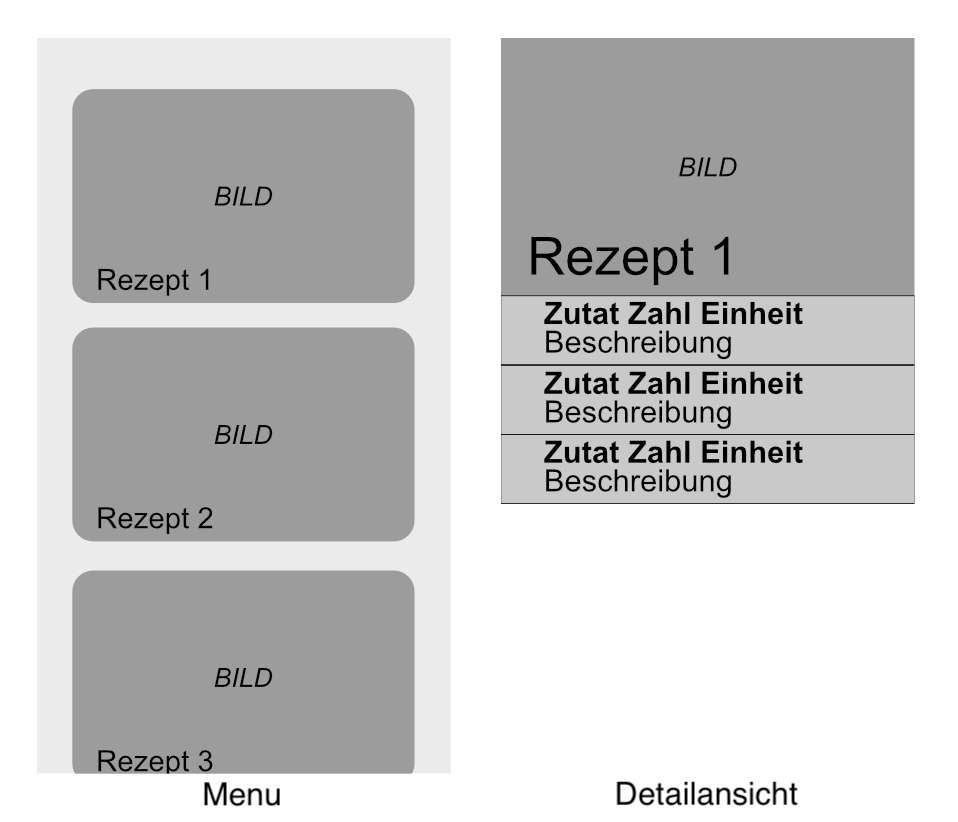
\includegraphics[width=\linewidth]{pictures/Sketch.png}
    \caption{Frühe Skizze}
    \label{fig:earlySketch}
\end{figure}
Nach diesen Überlegungen musste ich herausfinden woher ich Daten für die App, beziehungsweise die Kochrezepte, kriege und in welchem Format. So gelang ich mithilfe meines Vaters an Rezepte der V-ZUG AG in einem XML-Format. Ein XML-Format, ist eine bestimmte Form einer Datenansammlung, mehr dazu im nächsten Kapitel. Um diese XML-Dateien jedoch zu verwenden, müssen sie von der App zuerst noch eingelesen werden. Dies macht man, indem man es mithilfe eines sogennaten XML-Parsers, die XML-Datei in eine Struktur verwandelt, welche von Swift gelesen werden kann. Weiteres zum XML-Parser wird im folgenden Kapitel erklärt. 

\subsection{XML-Parser}
Der erste Schritt zur Kochapp fängt im sogenannten ,,Back-End`` an. Gemeint ist damit den Teil eines Programmcodes, mit welchem der Endnutzer nicht in Berührung kommt. In dem nachfolgenden Kapitel wird dann das ,,Front-End`` beschrieben, dabei handelt es sich um das Interface, mit welchem der Endnutzer konfrontiert wird und direkt zu Gesicht bekommt. Der Benutzer bemerkt das Back-End nie direkt. In diesem Fall ist das Back-End ein XML-Parser, dieser hat den Auftrag eine sogenannte XML-Datei für die App lesbar zu machen. Jedes Rezept wird in einer XML-Datei gespeichert. Eine XML-Datei ist eine spezielle Art von Datenstruktur, in welcher Informationen mithilfe von sogenannten ,,Tags`` gespeichert werden. Tags sind Objekte wie z.B. \colorbox{backcolour}{<lang>}, welche von einem schliessenden Tag geschlossen werden \colorbox{backcolour}{</lang>} (siehe gekürztes XML-Beispiel in Listing \ref{lst:xmlBsp}). \cite{bray2000extensible}
\begin{lstlisting}[language=XML,caption={XML-Beispiel gekürzt, Quelle: VZUG AG},label={lst:xmlBsp}]
<?xml version="1.0" encoding="UTF-8"?>
<tns:recipe xmlns:tns="http://vzug.ch/zughome/recipe-definition">
  <declarations>
      <device id="CS-SL-15">
        <recipe-id>
          <short-name>
            <lang ref="de">Confierter Lachs</lang>
          </short-name>
        </recipe-id>
      </device>
  </declarations>
</tns:recipe>
\end{lstlisting}
Die Information wird dann entweder innerhalb eines Tags gespeichert als \textit{Attribut} \colorbox{backcolour}{<device \textit{id=,,CS-SL-15``}>}. Oder \textit{zwischen} dem öffnenden Tag und dem schliessendem Tag \colorbox{backcolour}{<lang>\textit{Confierter Lachs}</lang>}. \\ Mit diesem Wissen wendete ich mich an den XML-Parser von Xcode, bzw. der Programmierumgebung für iOS-Apps. Das Problem besteht darin, dass es keinen XML-Parser gibt für Xcode, welcher eine XML-Datei einliest und eine Tabelle ausgibt, so wie es dies in z.B. Python gibt. Ein einfaches Beispiel eines Programmcode für einen XML-Parser ist dieser hier:
\begin{lstlisting}[language=Swift,caption={XML-Parser in Swift},label={lst:xmlParser}]
// Beispiel für eine Variable welche anzeigt ob ein Element geöffnet wurde oder nicht.
var shortNameElement = false

// Beispiel für eine Variable welche den ausgelesenen Wert temporär trägt
var elementName: String = ""

// Beispiel für eine Variable welche den ausgelesenen Wert temporär trägt und später in eine Struktur übertragen wird
var shortName: String = ""
  
// 1. - Element wurde geöffnet
func parser(_ parser: XMLParser, didStartElement elementName: String, namespaceURI: String?, qualifiedName qName: String?, attributes attributeDict: [String : String] = [:]) {
    if elementName == "short-name" {
        shortNameElement = true
    }
    self.elementName = elementName
}
    
// 2. - Element wurde geschlossen
 func parser(_ parser: XMLParser, didEndElement elementName: String, namespaceURI: String?, qualifiedName qName: String?) {
    if elementName == "short-name" {
        shortNameElement = false
    }
}
      
// 3. - Interpretiere die Daten im Element
func parser(_ parser: XMLParser, foundCharacters string: String) {
    let data = string.trimmingCharacters(in: CharacterSet.whitespacesAndNewlines)
    if (!data.isEmpty) {
        if self.elementName == "lang" && shortNameElement {
            shortName = data
        } 
    }
}
\end{lstlisting}
Das grundlegende Prinzip ist einfach, der Parser hat drei Funktionen, je nachdem wo der Parser sich befindet wird eine davon aufgerufen. Hier sind die drei Funktionen, oben im Programmcode mit den entsprechenden Nummern gekennzeichnet: 
\begin{enumerate}
\item Die erste der drei Funktionen wird aufgerufen, wenn ein Element geöffnet wurde und ändert so eine Variable auf den Wert ,,true``, sodass die dritte Funktion weiss, welches Element geöffnet wurde. 
\item Die zweite Funktion ändert die gleiche Variable wieder auf ,,false`` sobald das Element geschlossen wird. 
\item Die dritte Funktion interpretiert schlussendlich den Wert zwischen zwei Elementen und speichert diesen  in eine temporäre Variable. Diese Funktion weiss nur mithilfe der ersten und der zweiten Funktion welches Element gerade interpretiert wird. Attribute können in der ersten Funktion geprüft werden. 
\end{enumerate}
Nun haben wir eine Durcheinander von Variablen, welche vom Parser geschrieben wurden. Um dies zu ordnen werden all ausgelesenen Variablen in einer Struktur gespeichert. Eine Struktur ist eine Anordnung von Variablen in Swift (siehe Listing \ref{lst:struktur}).

\begin{lstlisting}[language=Swift,caption={Struktur für ein Rezept},label={lst:struktur}]
struct recipeStruct {
    var shortName: String = ""
    var prepTime: String = ""
    var cookingTime: String = ""
    var equipment: [String] = []
    var ingredientCategories: [(ingredientID: String, name: String, unit: String)] = [] //X: ingredientX[0: ID, 1: Name, 2: Unit]
    var tasks: [(groupTitle: String, tasks: [(message: String, ingredientID: String, minMax: [String])])] = [] //X: groupX[0: groupTitle, X: taskX[0: message, 1: ingredientID, 2: minMax[min,max]]]
}
\end{lstlisting}
Im XML-Parser wurden mir bereits die drei Variablen und die drei Arrays (ein Array ist etwas ähnliches wie eine Liste), bzw. geschachtelte Arrays, erstellt. Das heisst die können jetzt direkt in dieser Struktur gespeichert werden. So ist eine dieser Strukturen ein Rezept, also kann man alle Strukturen zu einem Array hinzufügen und man erhält eine Liste von Rezepten. Diese Liste kann nun direkt vom Front-End iteriert werden und angezeigt werden. Das Bild ist gleichnamig wie das Rezept, also kann man die Variable ,,shortName`` benutzen um das zugehörige Bild anzuzeigen. Da die Struktur der XML-Datei viel komplexer ist als das Beispiel (siehe Listing \ref{lst:xmlParser}), werden auch viel mehr spezifische Variablen erstellt werden. Im Endeffekt muss ein XML-Parser in Swift genau auf die zu erwartende XML-Dateistruktur angepasst werden. Denn je nachdem was man auslesen will, müssen andere Variabeln gewählt werden. Im nachfolgenden Kapitel wird das Front-End erklärt. \cite{xmlParserIosCreator}

\subsection{UITableView}
Im vorherigen Kapitel wurden die Daten bereit gemacht um dargestellt zu werden. Die Rezepte befinden sich nun in einem Array von Strukturen. Was ist eine ,,UITableView``? Jeder von uns hat eine solche bereits verwendet, es gibt sie auf Android sowie iOS. UITableViews sind einfache Listen. Sie bestehen aus zwei Komponenten. Der eine Teil ist die UITableView selbst und der zweite eine UITableViewCell (siehe Abb. \ref{fig:TableView}), also eine ,,Zelle` analog aus Tabellen. 
\begin{figure}
    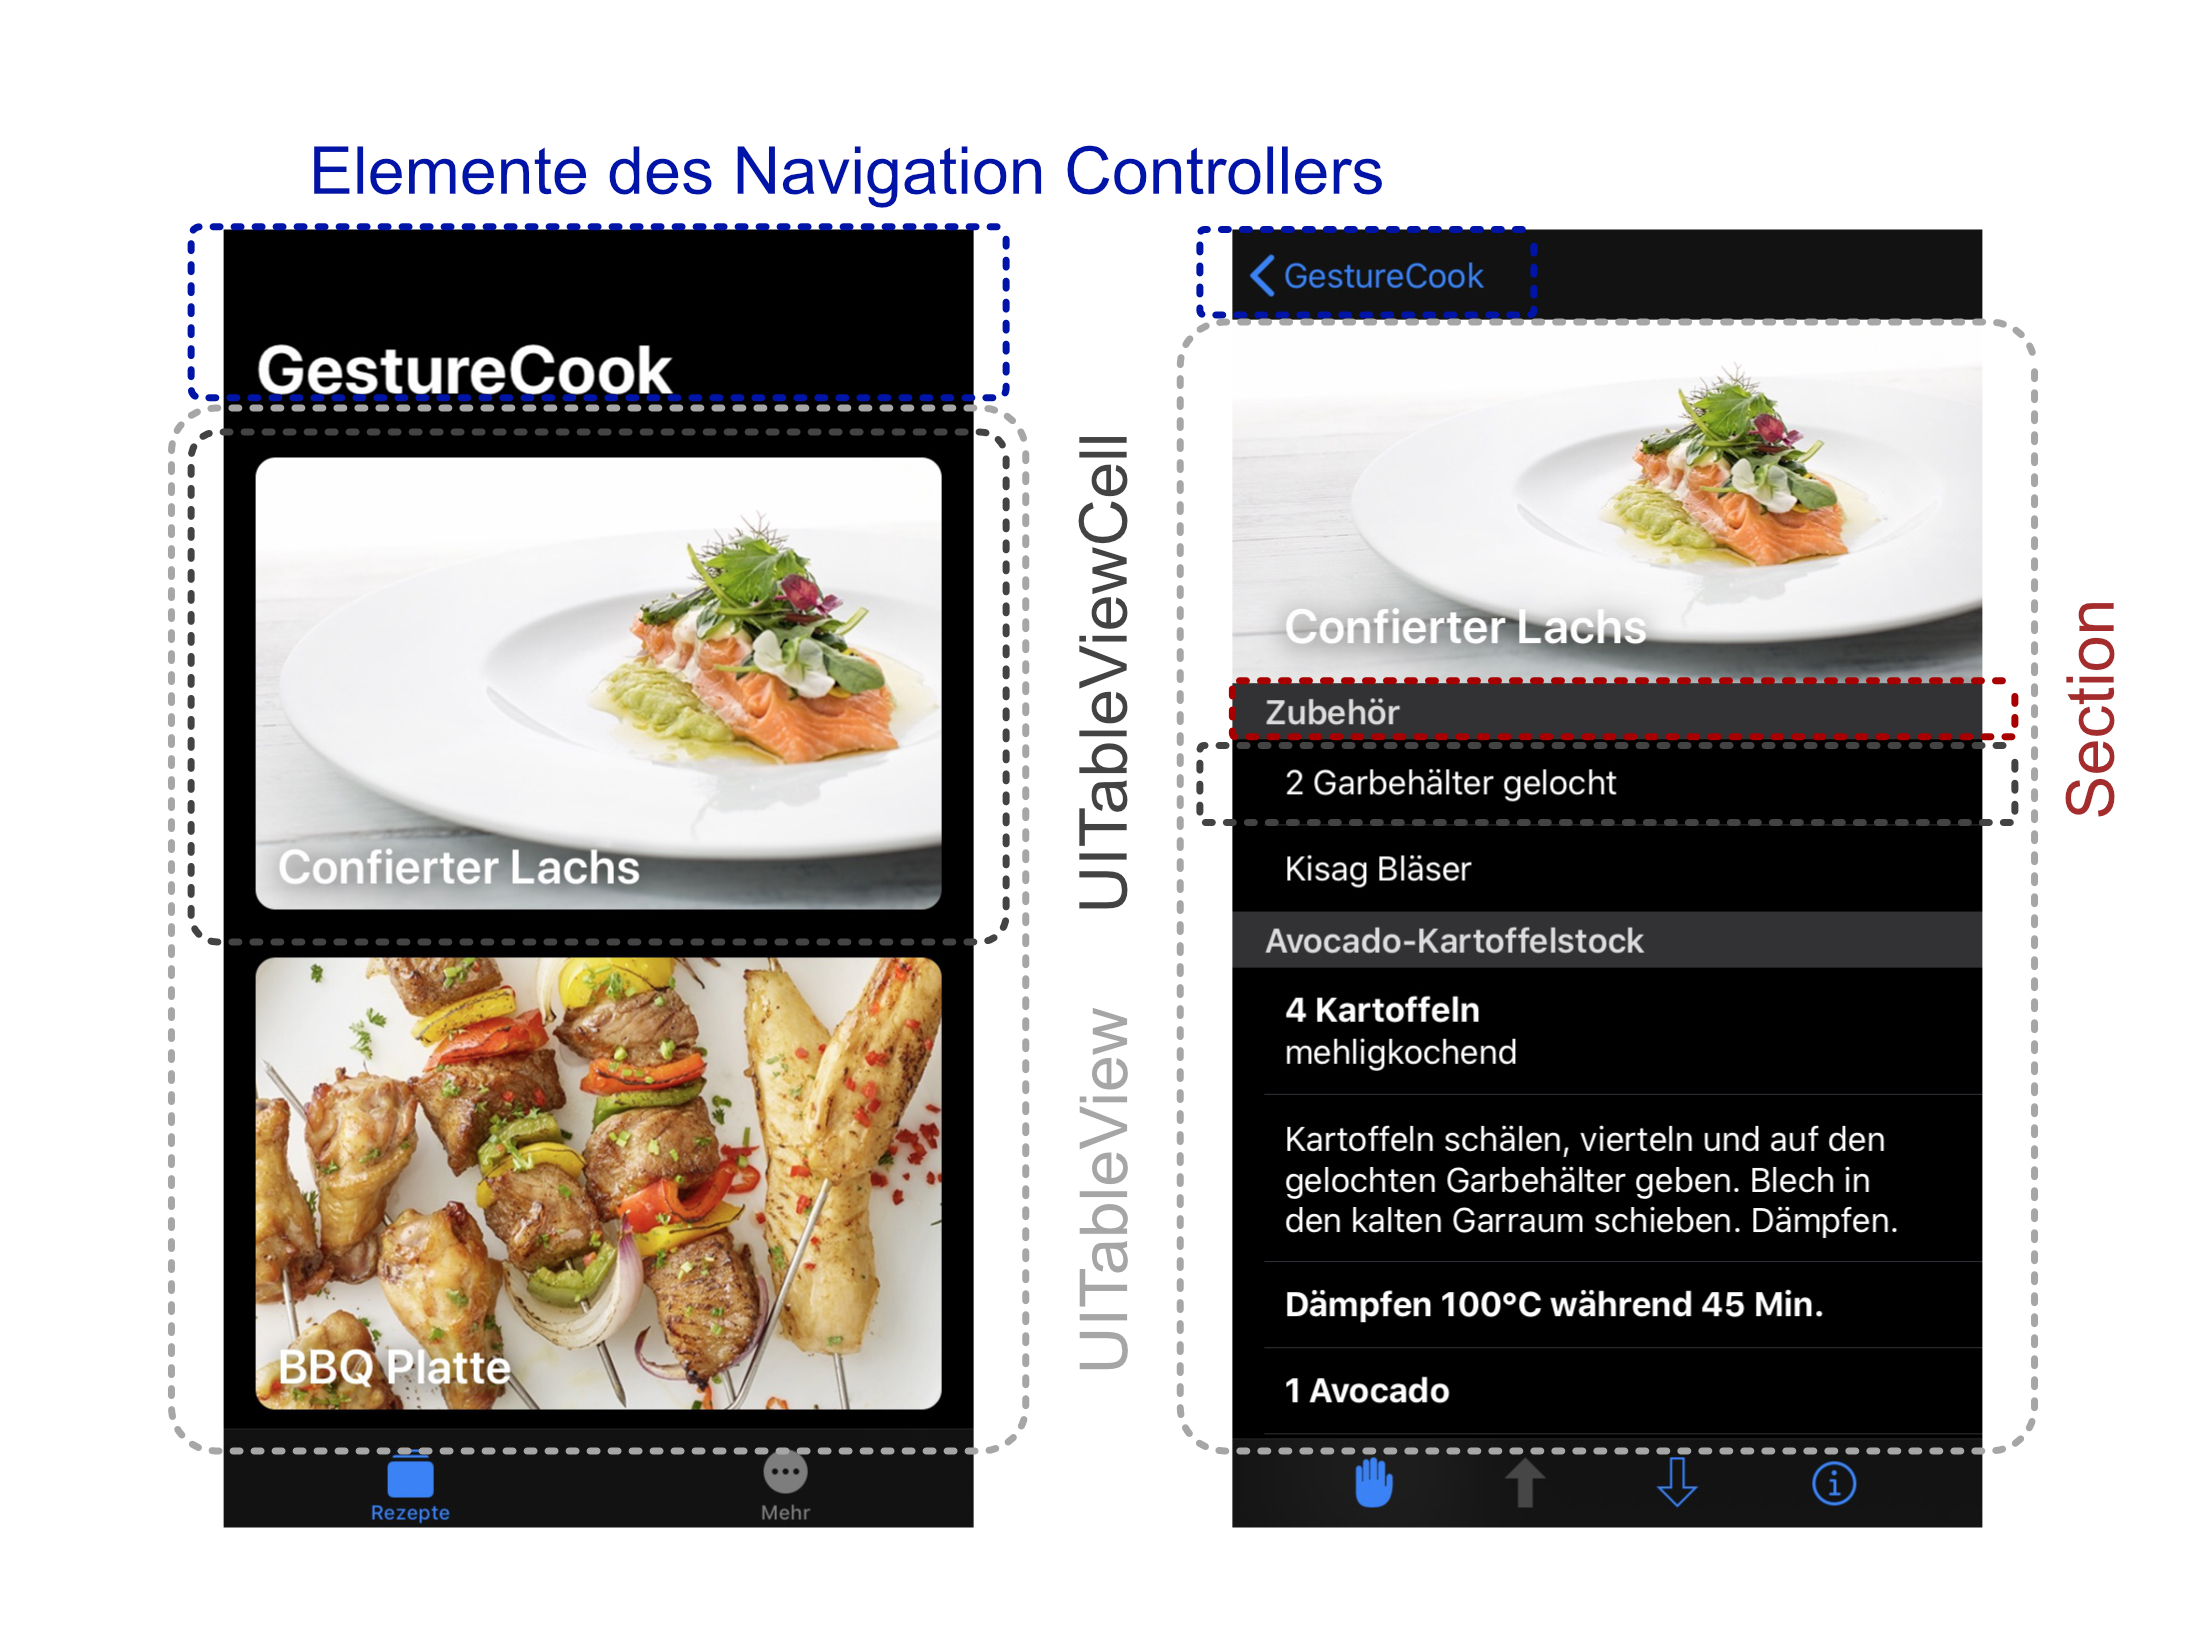
\includegraphics[width=\linewidth]{pictures/TableView.jpg}
    \caption{Komponente der TableView}
    \label{fig:TableView}
\end{figure}
Solche UITableViews können auch in Sections eingeteilt werden. Praktisch ist, dass das Design von Xcode erstellt wird. Sogar die Steuerung, bzw. das Scrollen und die Navigation übernimmt Xcode. Denn wenn man eine UITableView importiert, kommt diese automatisch mit einem Navigation Controller. Dieser übernimmt einem die Arbeit von Knöpfen die einen Bildschirm zurückgehen, oder einen Titel auf der Oberseite des Bildschirms. \\ Allerdings kann nicht alles automatisch erstellt werden, denn eine normale UITableViewCell ist eine Zelle mit einem Label (ein Text) im Innern. Um Bilder oder mehrere Labels, bei welchen die eine z.B. fett geschrieben ist, in einer Zelle zu erstellen (siehe Abb.  \ref{fig:earlySketch}), braucht es CustomUITableViewCells. Diese kann man einmal erstellen und dann tausendfach mit verschiedenem Inhalt anzeigen lassen. Diese Möglichkeit erlaubt es einem nun durch die vorher kreierte Liste zu iterieren und so jeden Schritt des Rezeptes, sowie des Titels mit Bild, anzuzeigen. Die Bilder sind wie die Rezepte lokal in der App gespeichert und können nun mithilfe des Rezepte-Namens aufgerufen werden. \cite{tableviewvideo,tableViewApple}

\subsection{Künstliche Intelligenz trainieren}
Bis hierhin wurde erklärt wie man eine voll funktionale Rezepte-App erstellt. Allerdings fehlt noch der wichtigste Teil der App, die Gestensteuerung. Das Ziel ist es, die Library ,,Core ML`` von Apple zu verwenden um die Künstliche Intelligenz zu trainieren und damit den Output der Frontkamera auszuwerten. Das ,,ML`` steht für ,,Machine Learning`` also Maschinelles Lernen. Diese Bezeichnung ist sehr passend, denn tatsächlich muss die KI zuerst ,,lernen`` um akkurate Ergebnisse zu erzielen. Gerade mithilfe Core ML ist dies ein sehr einfacher Prozess, denn es gibt sogar eine Applikation von Apple namens ,,Create ML``, welche einem beim Trainieren hilft (siehe Abb. \ref{fig:createML}). In diesem Fall soll die Gestensteuerung wie folgt funktionieren: Sobald der Benutzer die Hand über die Kamera hält und eine Faust formt, soll die App nach unten scrollen. Wenn der Nutzer die Hand wieder wegnimmt soll es aufhören zu scrollen. Mit weit gespreizter Hand, kann er nun wieder nach oben scrollen. \\ So soll die KI zwischen drei Fällen unterscheiden, erstens einer Faust, zweitens einer gespreizten Hand und drittens ,,Nichts``. ,,Nichts`` für den  Fall, dass der Nutzer die Hand nicht über der Kamera hält, also keine Aktion gestartet werden soll. Man ,,füttert`` nun die Künstliche Intelligenz mit einfachen Bildern. Also nimmt man Bilder von vielen Fäusten, gespreizten Händen und von leeren Hintergründen auf (für Beispiele siehe Abb. \ref{fig:qualityoftraining}). Diesen Prozess nennt man Klassifizierung, also wird der Künstlichen Intelligenz erklärt, auf welchen Bildern was zu erkennen ist. Innerhalb der Create ML Applikation kann man nun drei Ordner mit dem Namen der drei Fälle und den zugehörigen Bildern importieren, diese werden dann von der Künstlichen Intelligenz analysiert. \\ Doch nur das Training ohne Auswertung hat keine Bedeutung, man weiss nicht, ob die Künstliche Intelligenz funktioniert oder nicht. Deshalb macht man weitere Fotos von diesen drei Fällen, welche die KI noch nie gesehen hat und lässt diese von der KI evaluieren. So bekam ich mit insgesamt 707 Bildern eine Genauigkeit von 91\% (siehe Abb. \ref{fig:createML}) was weitaus genug genau für Gestensteuerung ist, mehr dazu im nächsten Kapitel. Links in der Abbildung \ref{fig:createML} sieht man die verschiedenen Versionen meiner KI-Dateien. In der Mitte sieht man die drei Kategorien (Faust, gespreitzte Hand und Nichts) und die Genauigkeit der Abschätzung in diesen Kategorien. \cite{gesturecontrolvideo}\\
\begin{figure}
    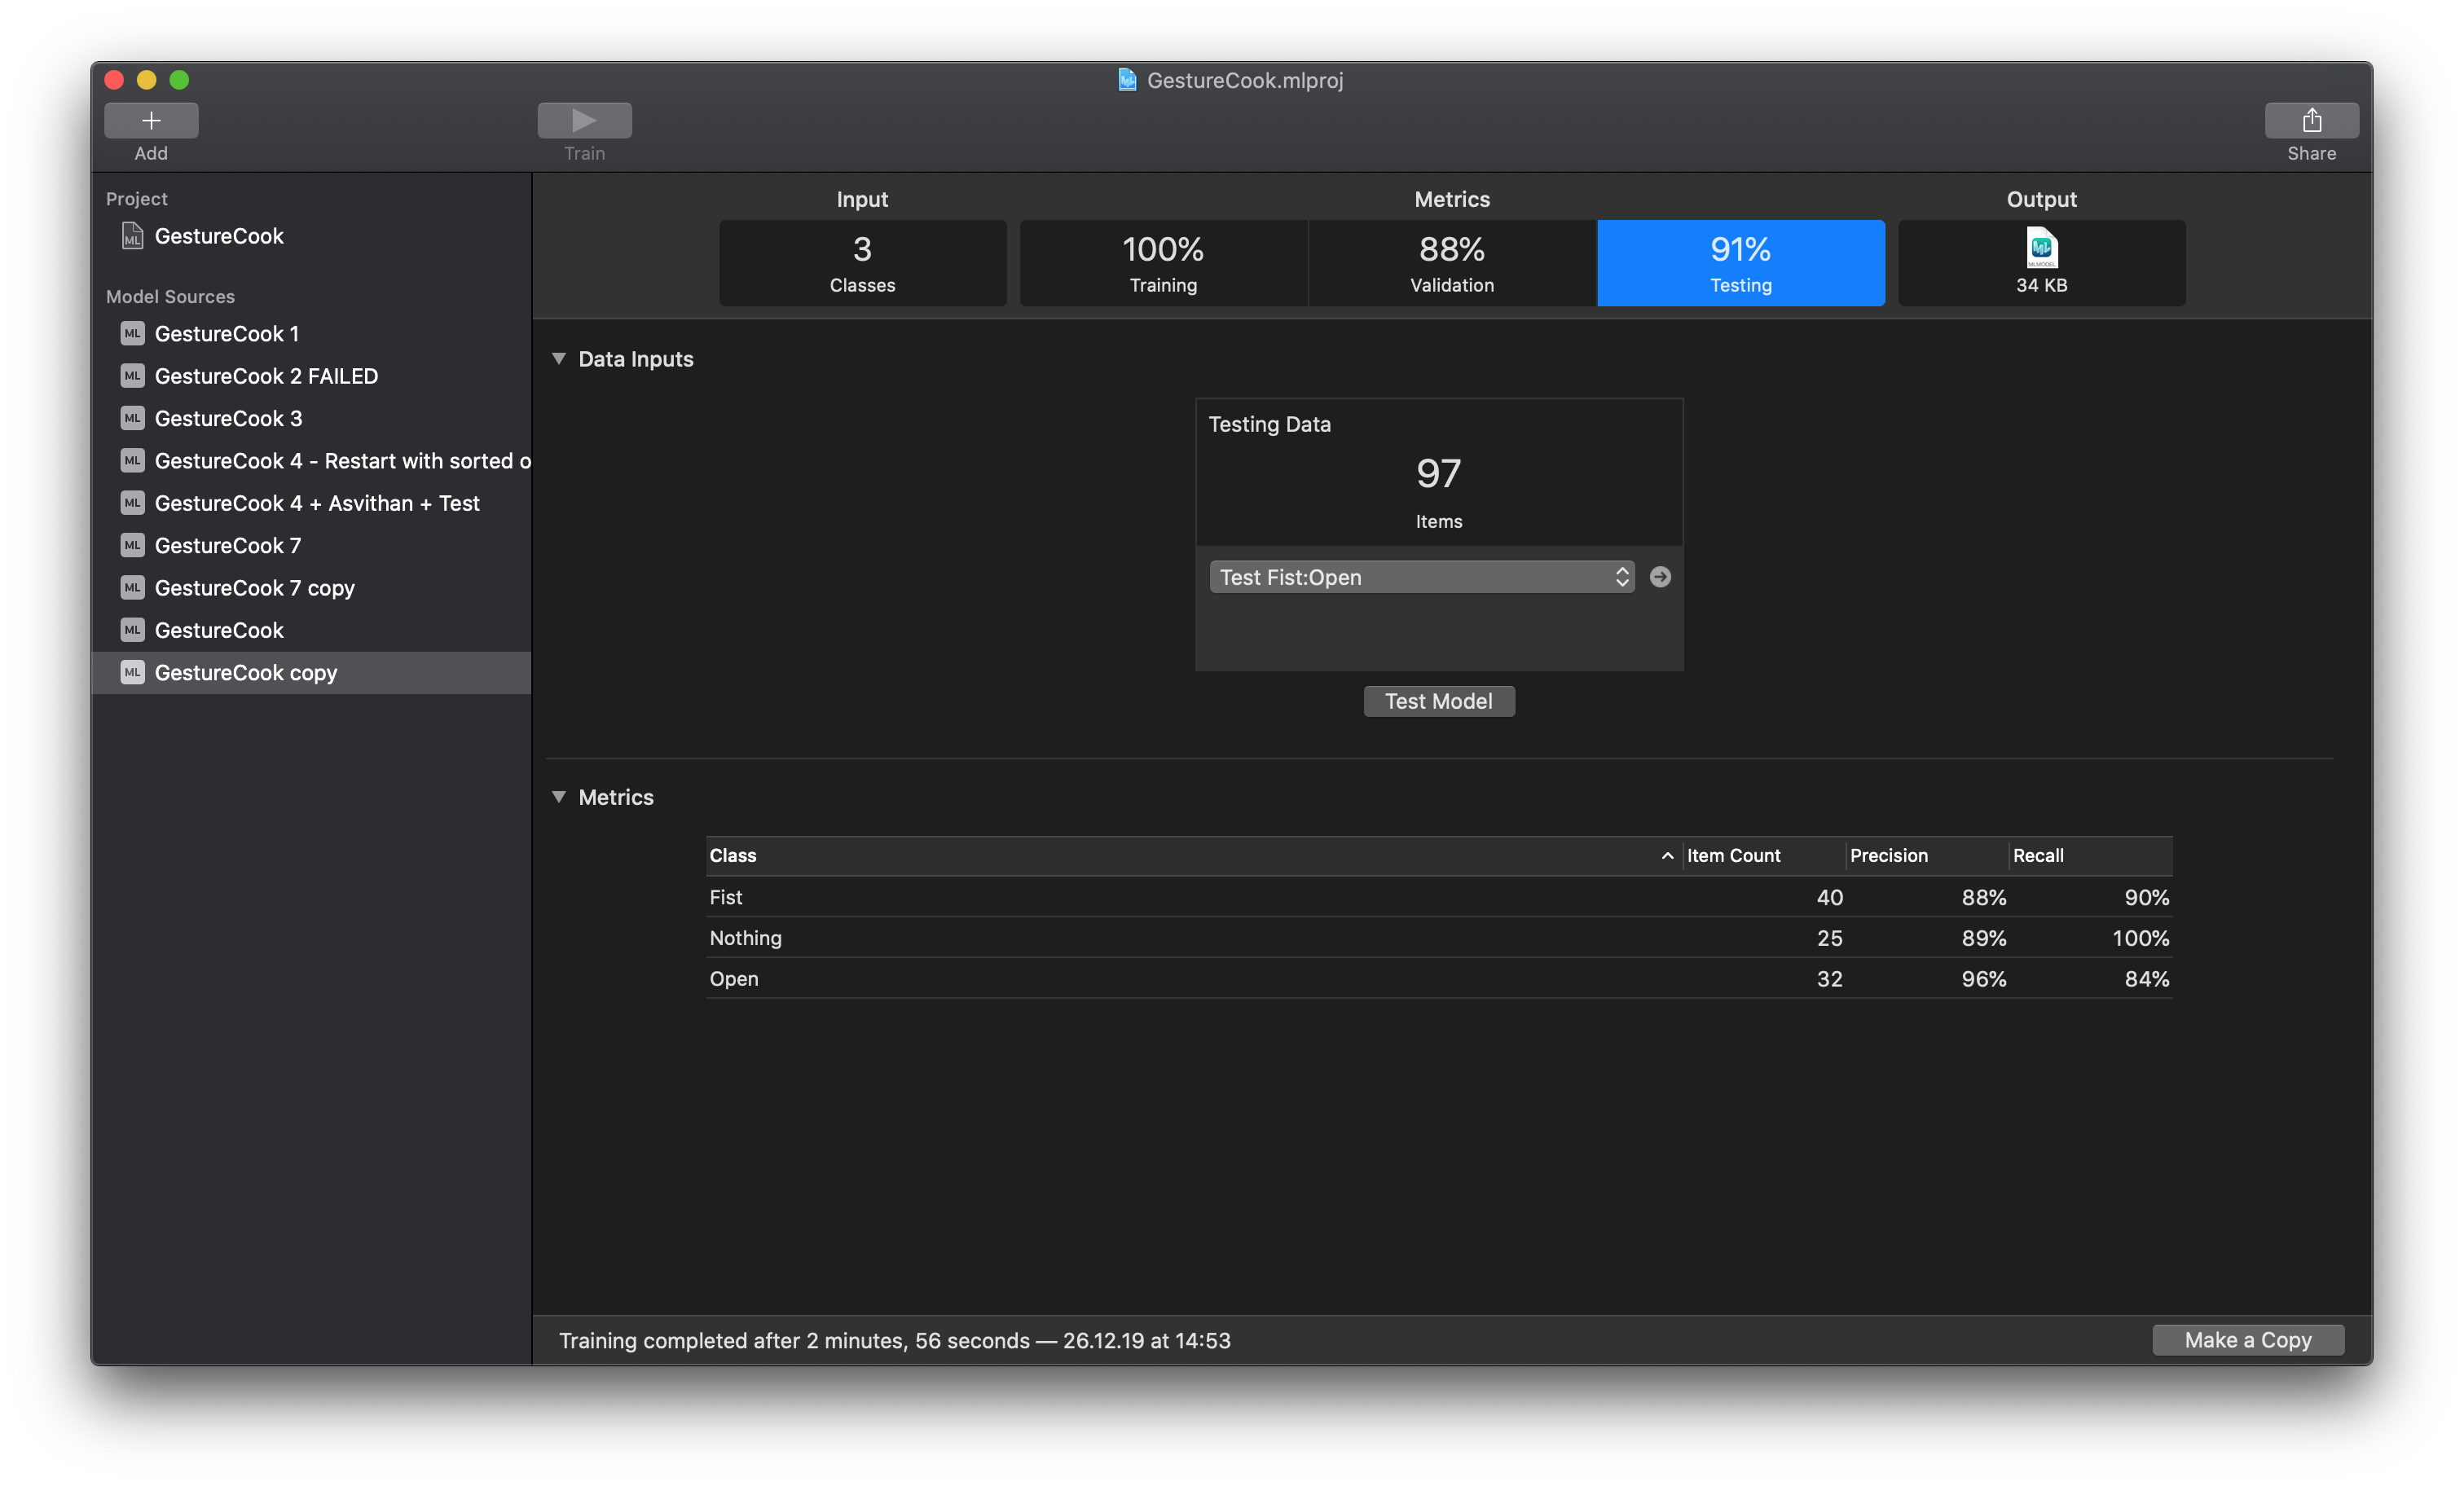
\includegraphics[width=\linewidth]{pictures/CreateML.png}
    \caption{Create ML Testresultat nach ungefähr 700 Bildern}
    \label{fig:createML}
\end{figure}
Doch diese 90\% erhielt ich erst nach vielen Fehlversuchen. Anfangs war die Idee, als Gesten für hoch und runter den Daumen nach oben, bzw. nach unten zu definieren. Dies stellte sich allerdings als beinahe unerkennbar für die KI heraus. Mit ganzen 746 Bildern erhielt ich eine Genauigkeit von nur 45\%, dies ist zu ungenau für eine Unterscheidung von drei Fällen. Ich versuchte die Bilder in möglichst vielen verschiedenen Lichtsituationen aufzunehmen, denn die KI sollte in vielen verschiedenen Umgebungen funktionieren. Einer meiner Fehler war auch mit den neuen Gesten, die fehlende Qualität der Bilder. Auch wenn unklare Bilder die KI verbessern kann, können diese auch zu unklar sein. Entweder war die Handgeste nicht genug eindeutig (siehe Abb. \ref{fig:unklargeste}) oder die Lichtverhältnisse sind zu schlecht, damit die KI das Bild erkennt (siehe Abb. \ref{fig:unklarlicht}). Ich stellte sicher, dass die Gesten auch für einen Menschen klar erkennbar sind (siehe Beispiele Abb. \ref{fig:klarfaust} und \ref{fig:klaroffen}), denn falls dies nicht der Fall ist, verwirrt dieses Bild die KI. So bin ich zum Schluss gekommen, dass der Fokus auf Qualität des Trainingsmaterials wichtig ist. Erstaunlicherweise funktionierte die KI sehr gut bei meinem dunkelhäutigen Kollegen, ohne dass ein Bild einer dunkelhäutigen Hand in den Trainingsdaten vorhanden war. In der finalen Version allerdings wurden auch dunkelhäutige Hände als Trainingsdaten verwendet um eine möglichst akkurate Schätzung zu erzeugen. \\ Das trainieren der KI startet mit einem einfachen Knopfdruck (siehe Abb. \ref{fig:createML} oben links "Train") und dauert nur wenige Minuten. Als Resultat der fertig trainierten KI erhält man eine Datei mit dem Suffix ,,.mlmodel``, welche erstaunlicherweise nur um die 34 Kilobyte gross ist.
\begin{figure*}
        \centering
        \begin{subfigure}[b]{0.475\textwidth}
            \centering
            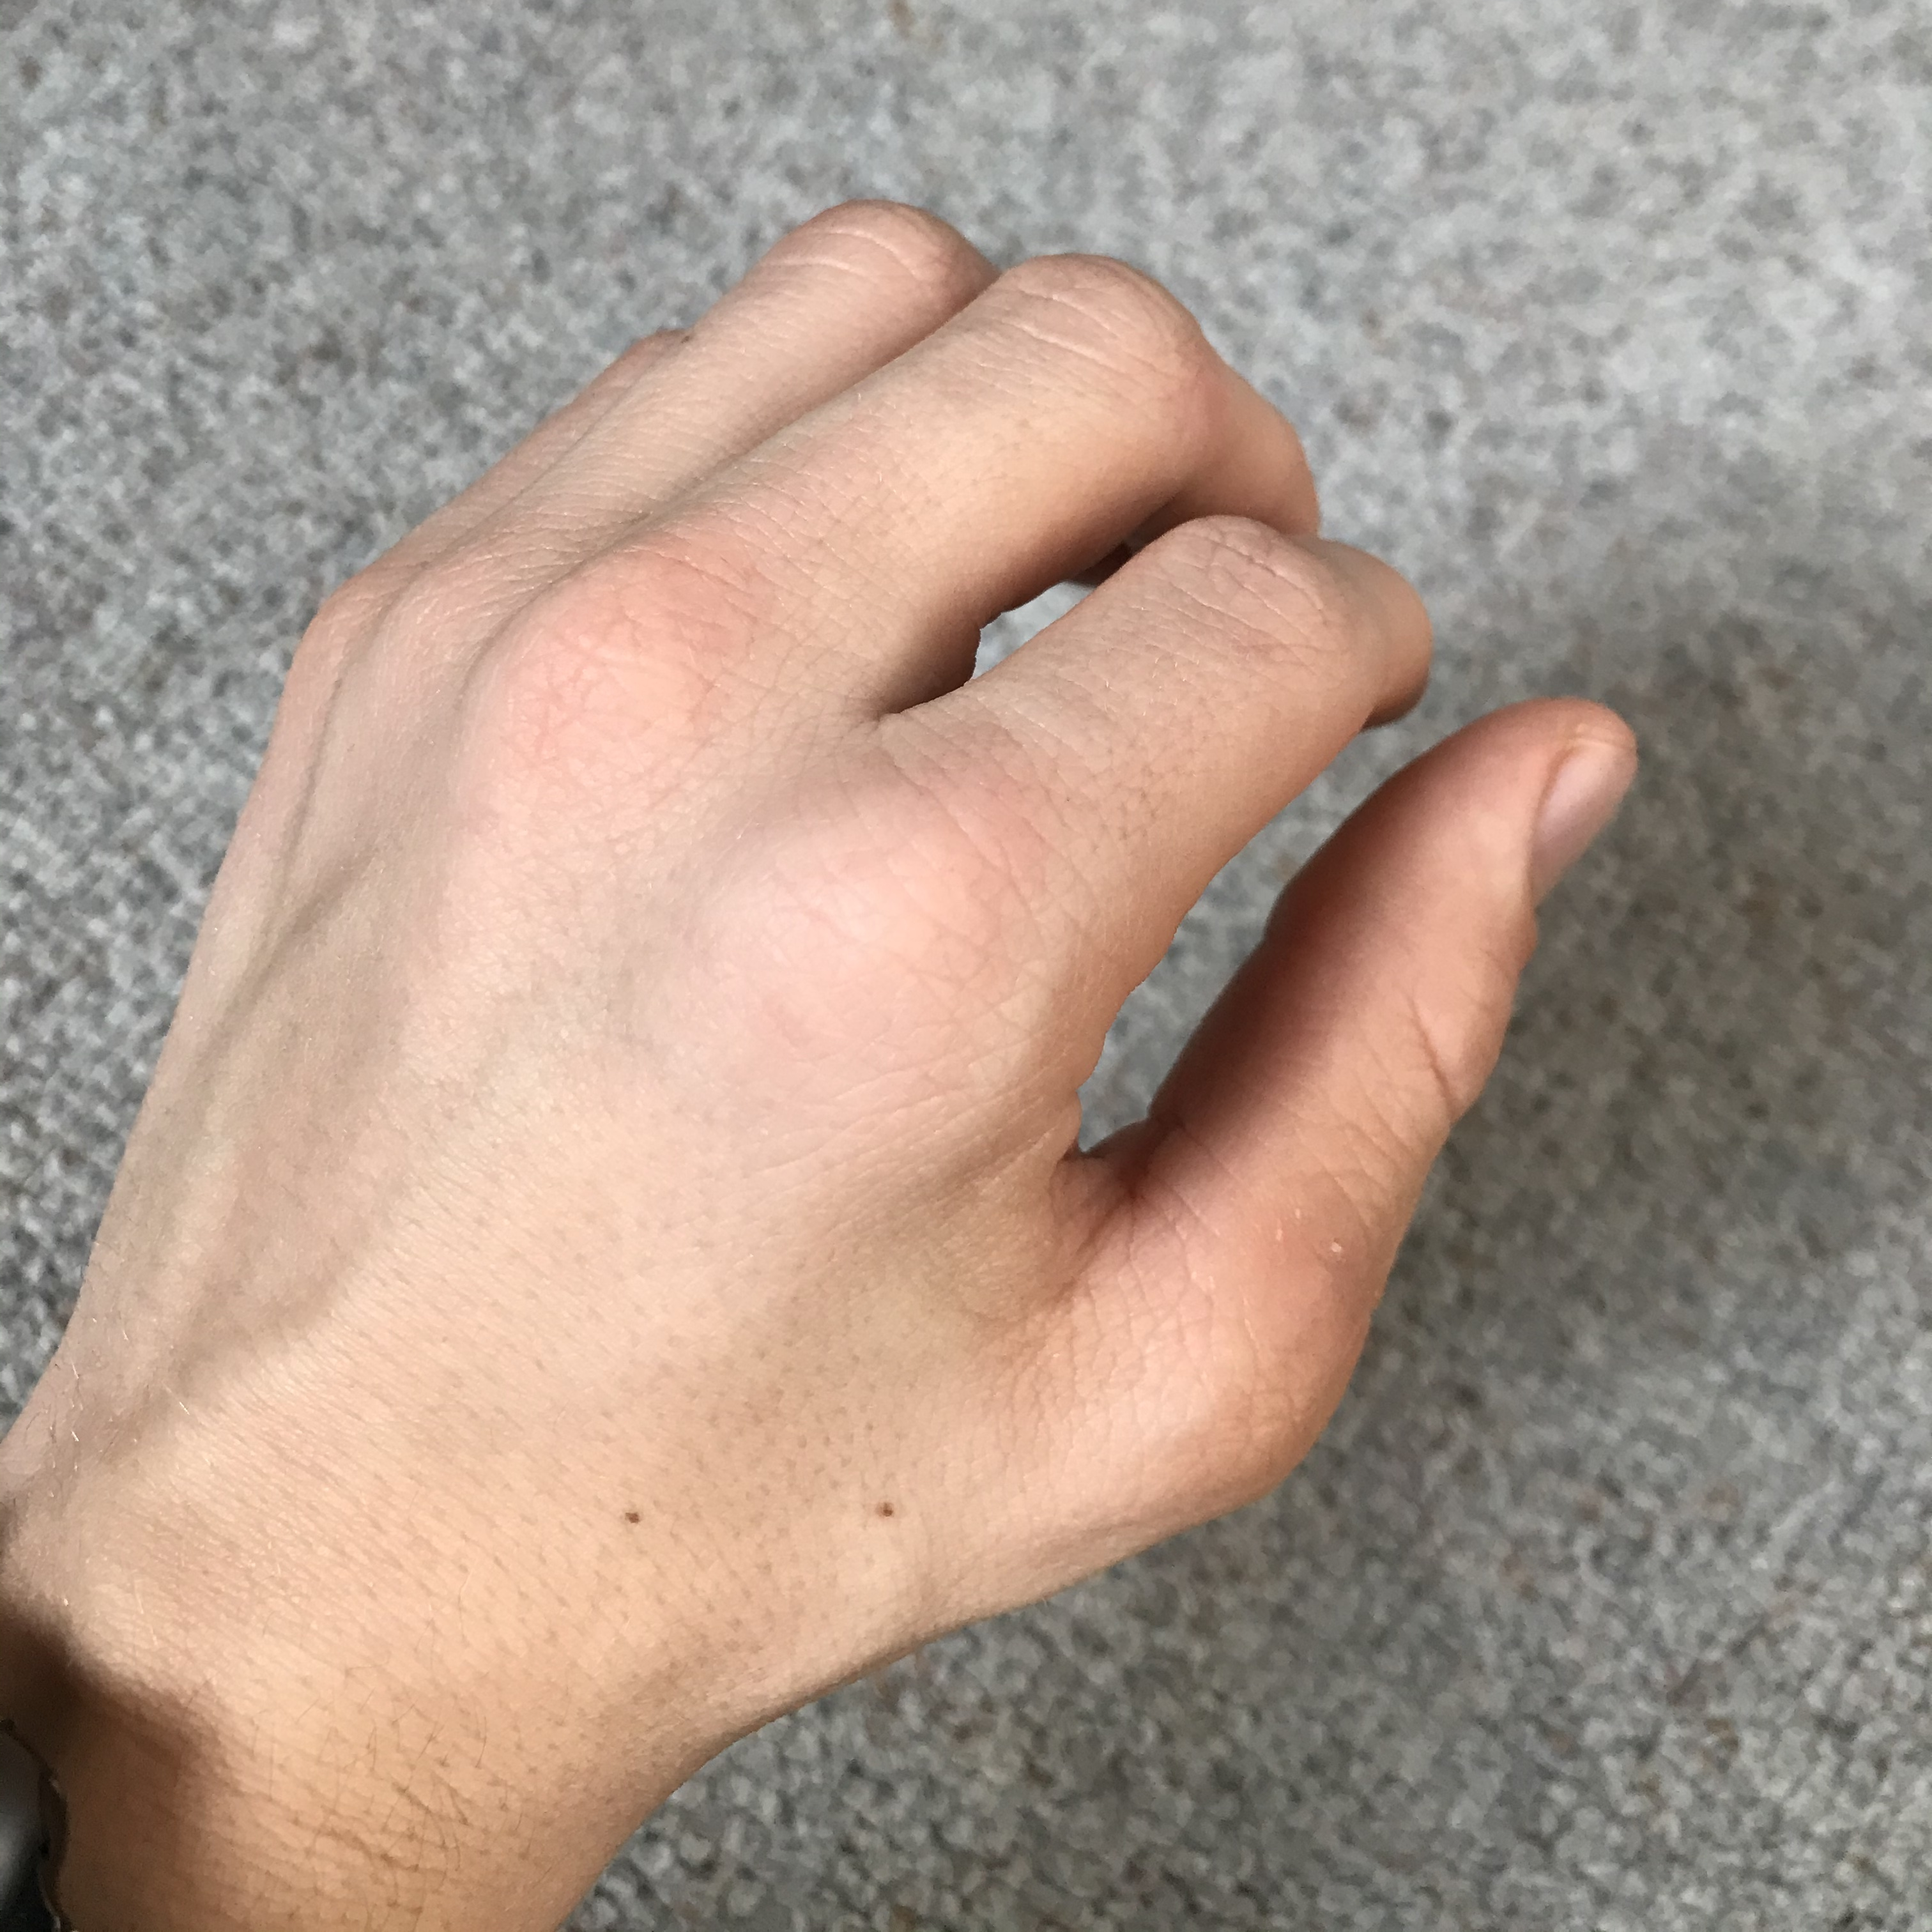
\includegraphics[width=\textwidth]{pictures/unklargeste.jpg}
            \caption[]%
            {{\small Bild scharf, aber Geste unklar}}    
            \label{fig:unklargeste}
        \end{subfigure}
        \hfill
        \begin{subfigure}[b]{0.475\textwidth}  
            \centering 
            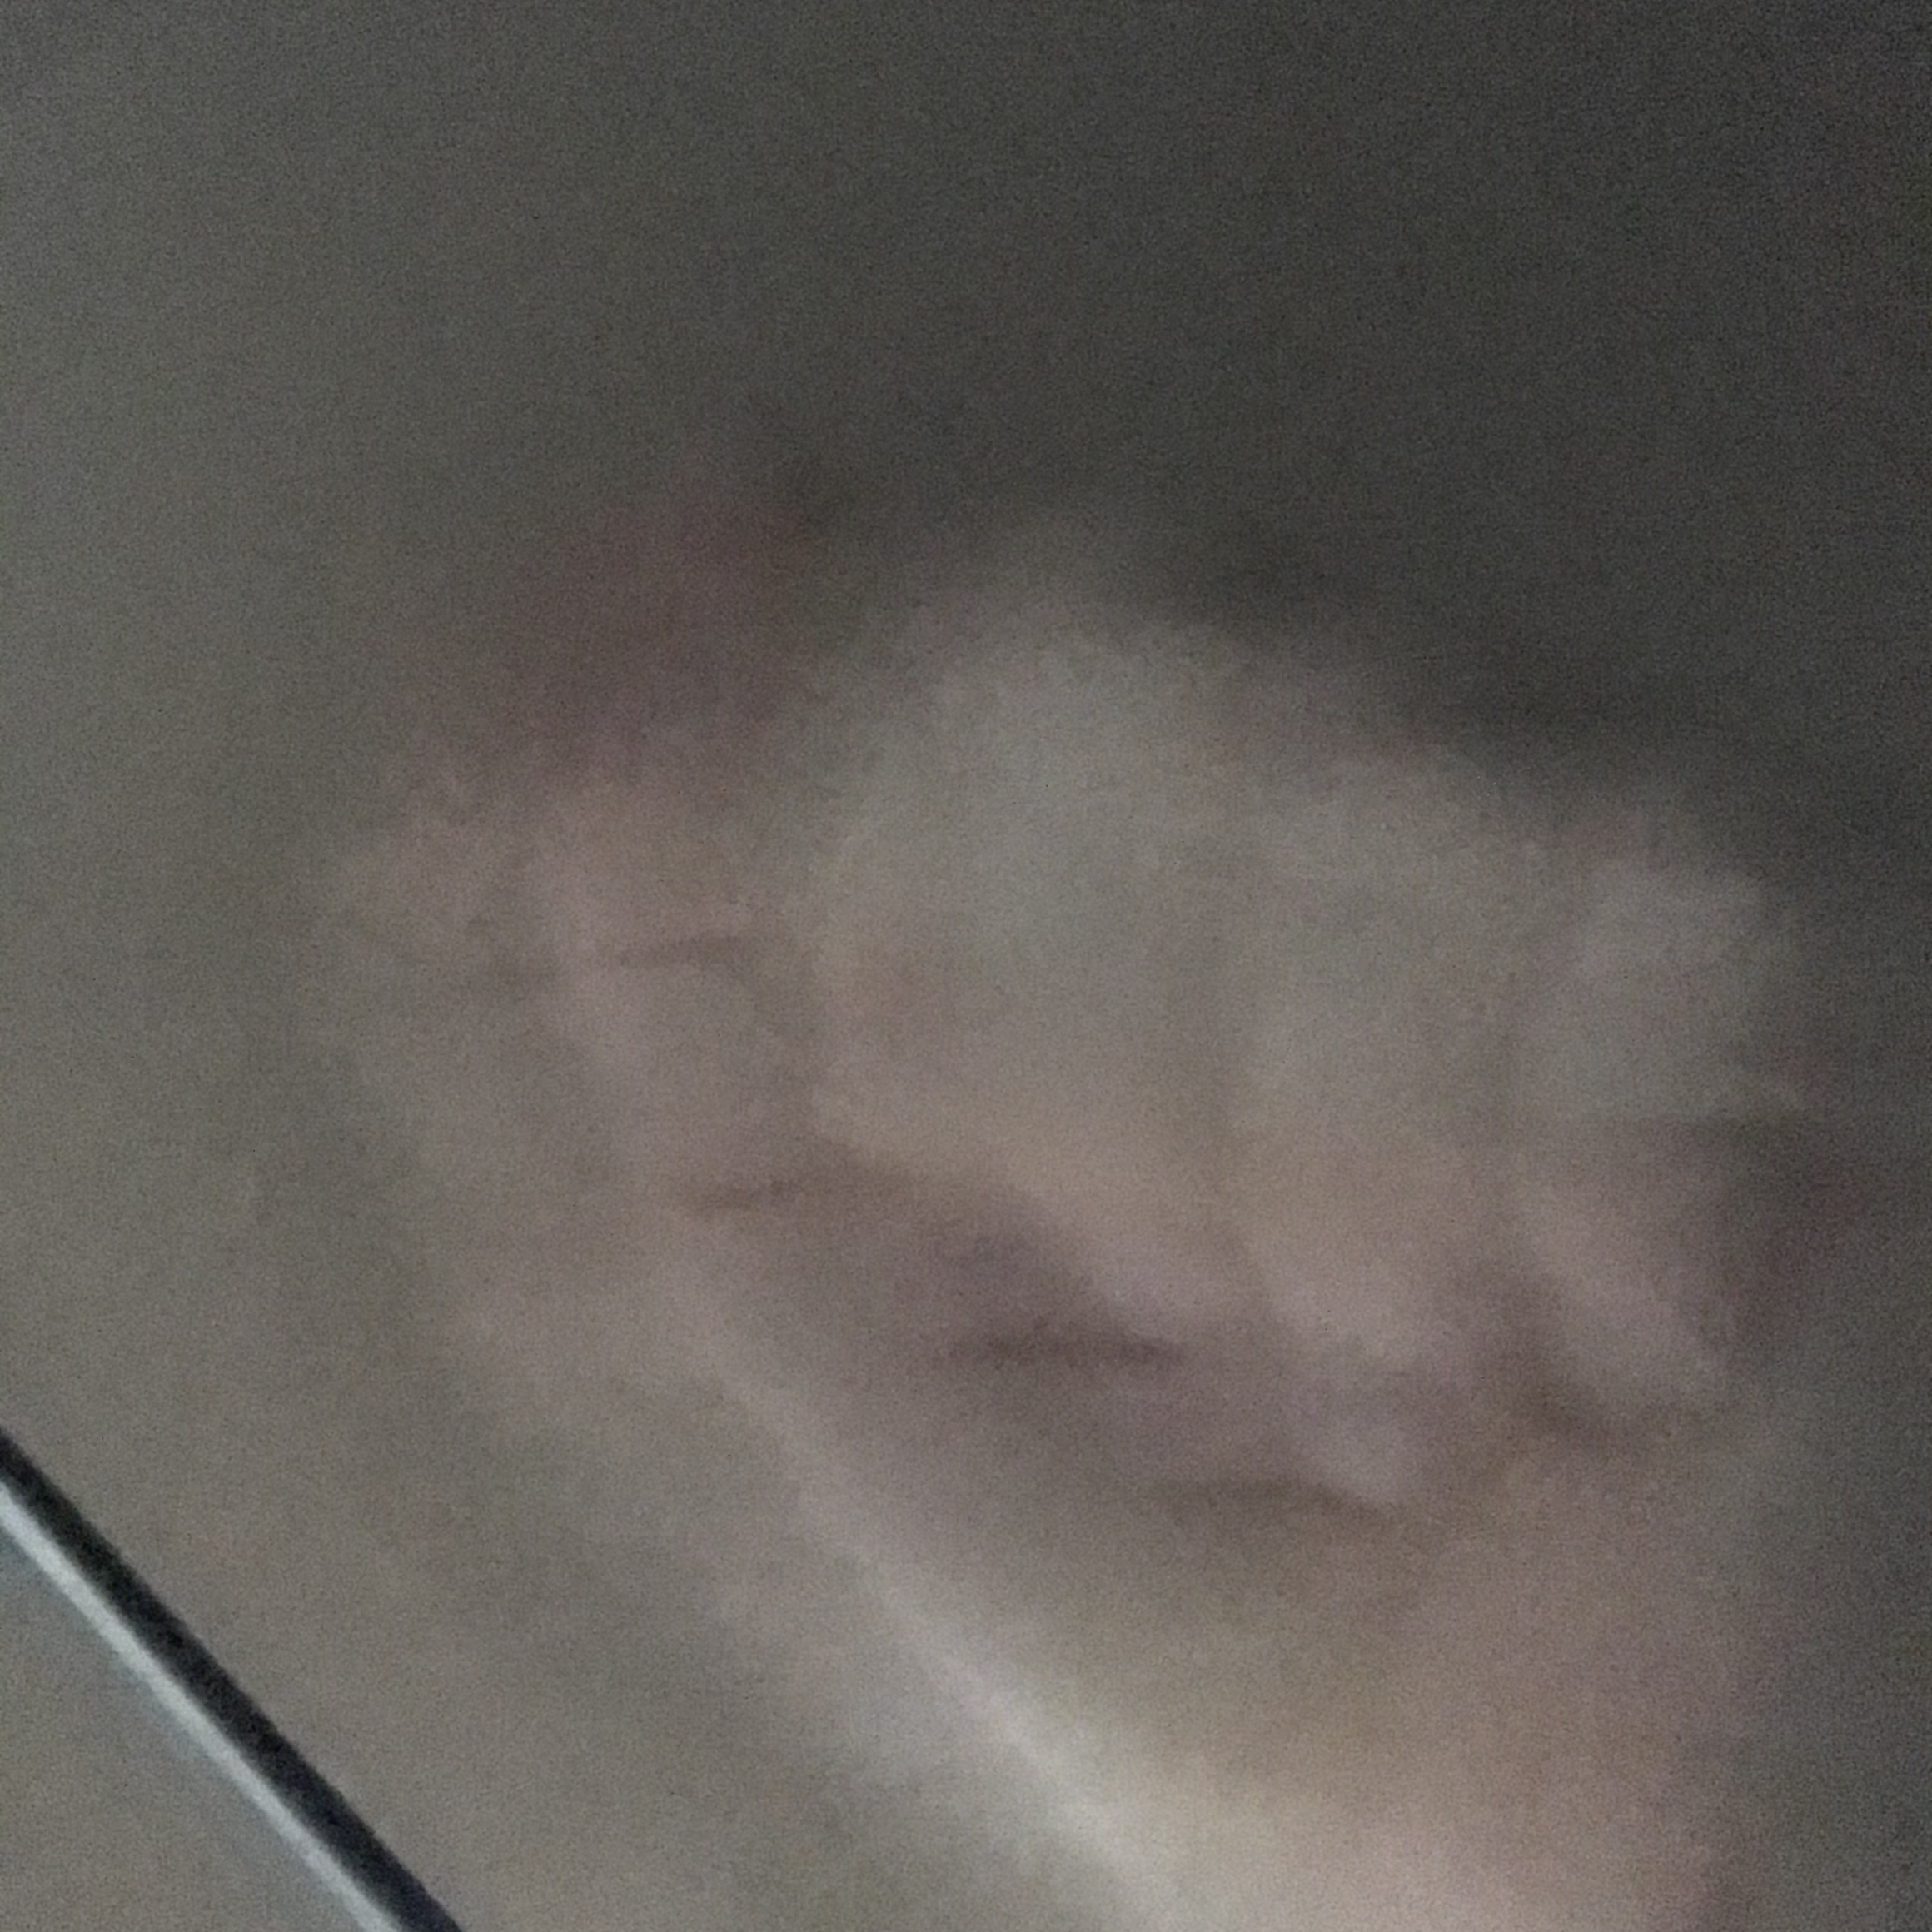
\includegraphics[width=\textwidth]{pictures/unklarlicht.jpg}
            \caption[]%
            {{\small Lichtverhältnisse schlecht, unklar}}    
            \label{fig:unklarlicht}
        \end{subfigure}
        \vskip\baselineskip
        \begin{subfigure}[b]{0.475\textwidth}   
            \centering 
            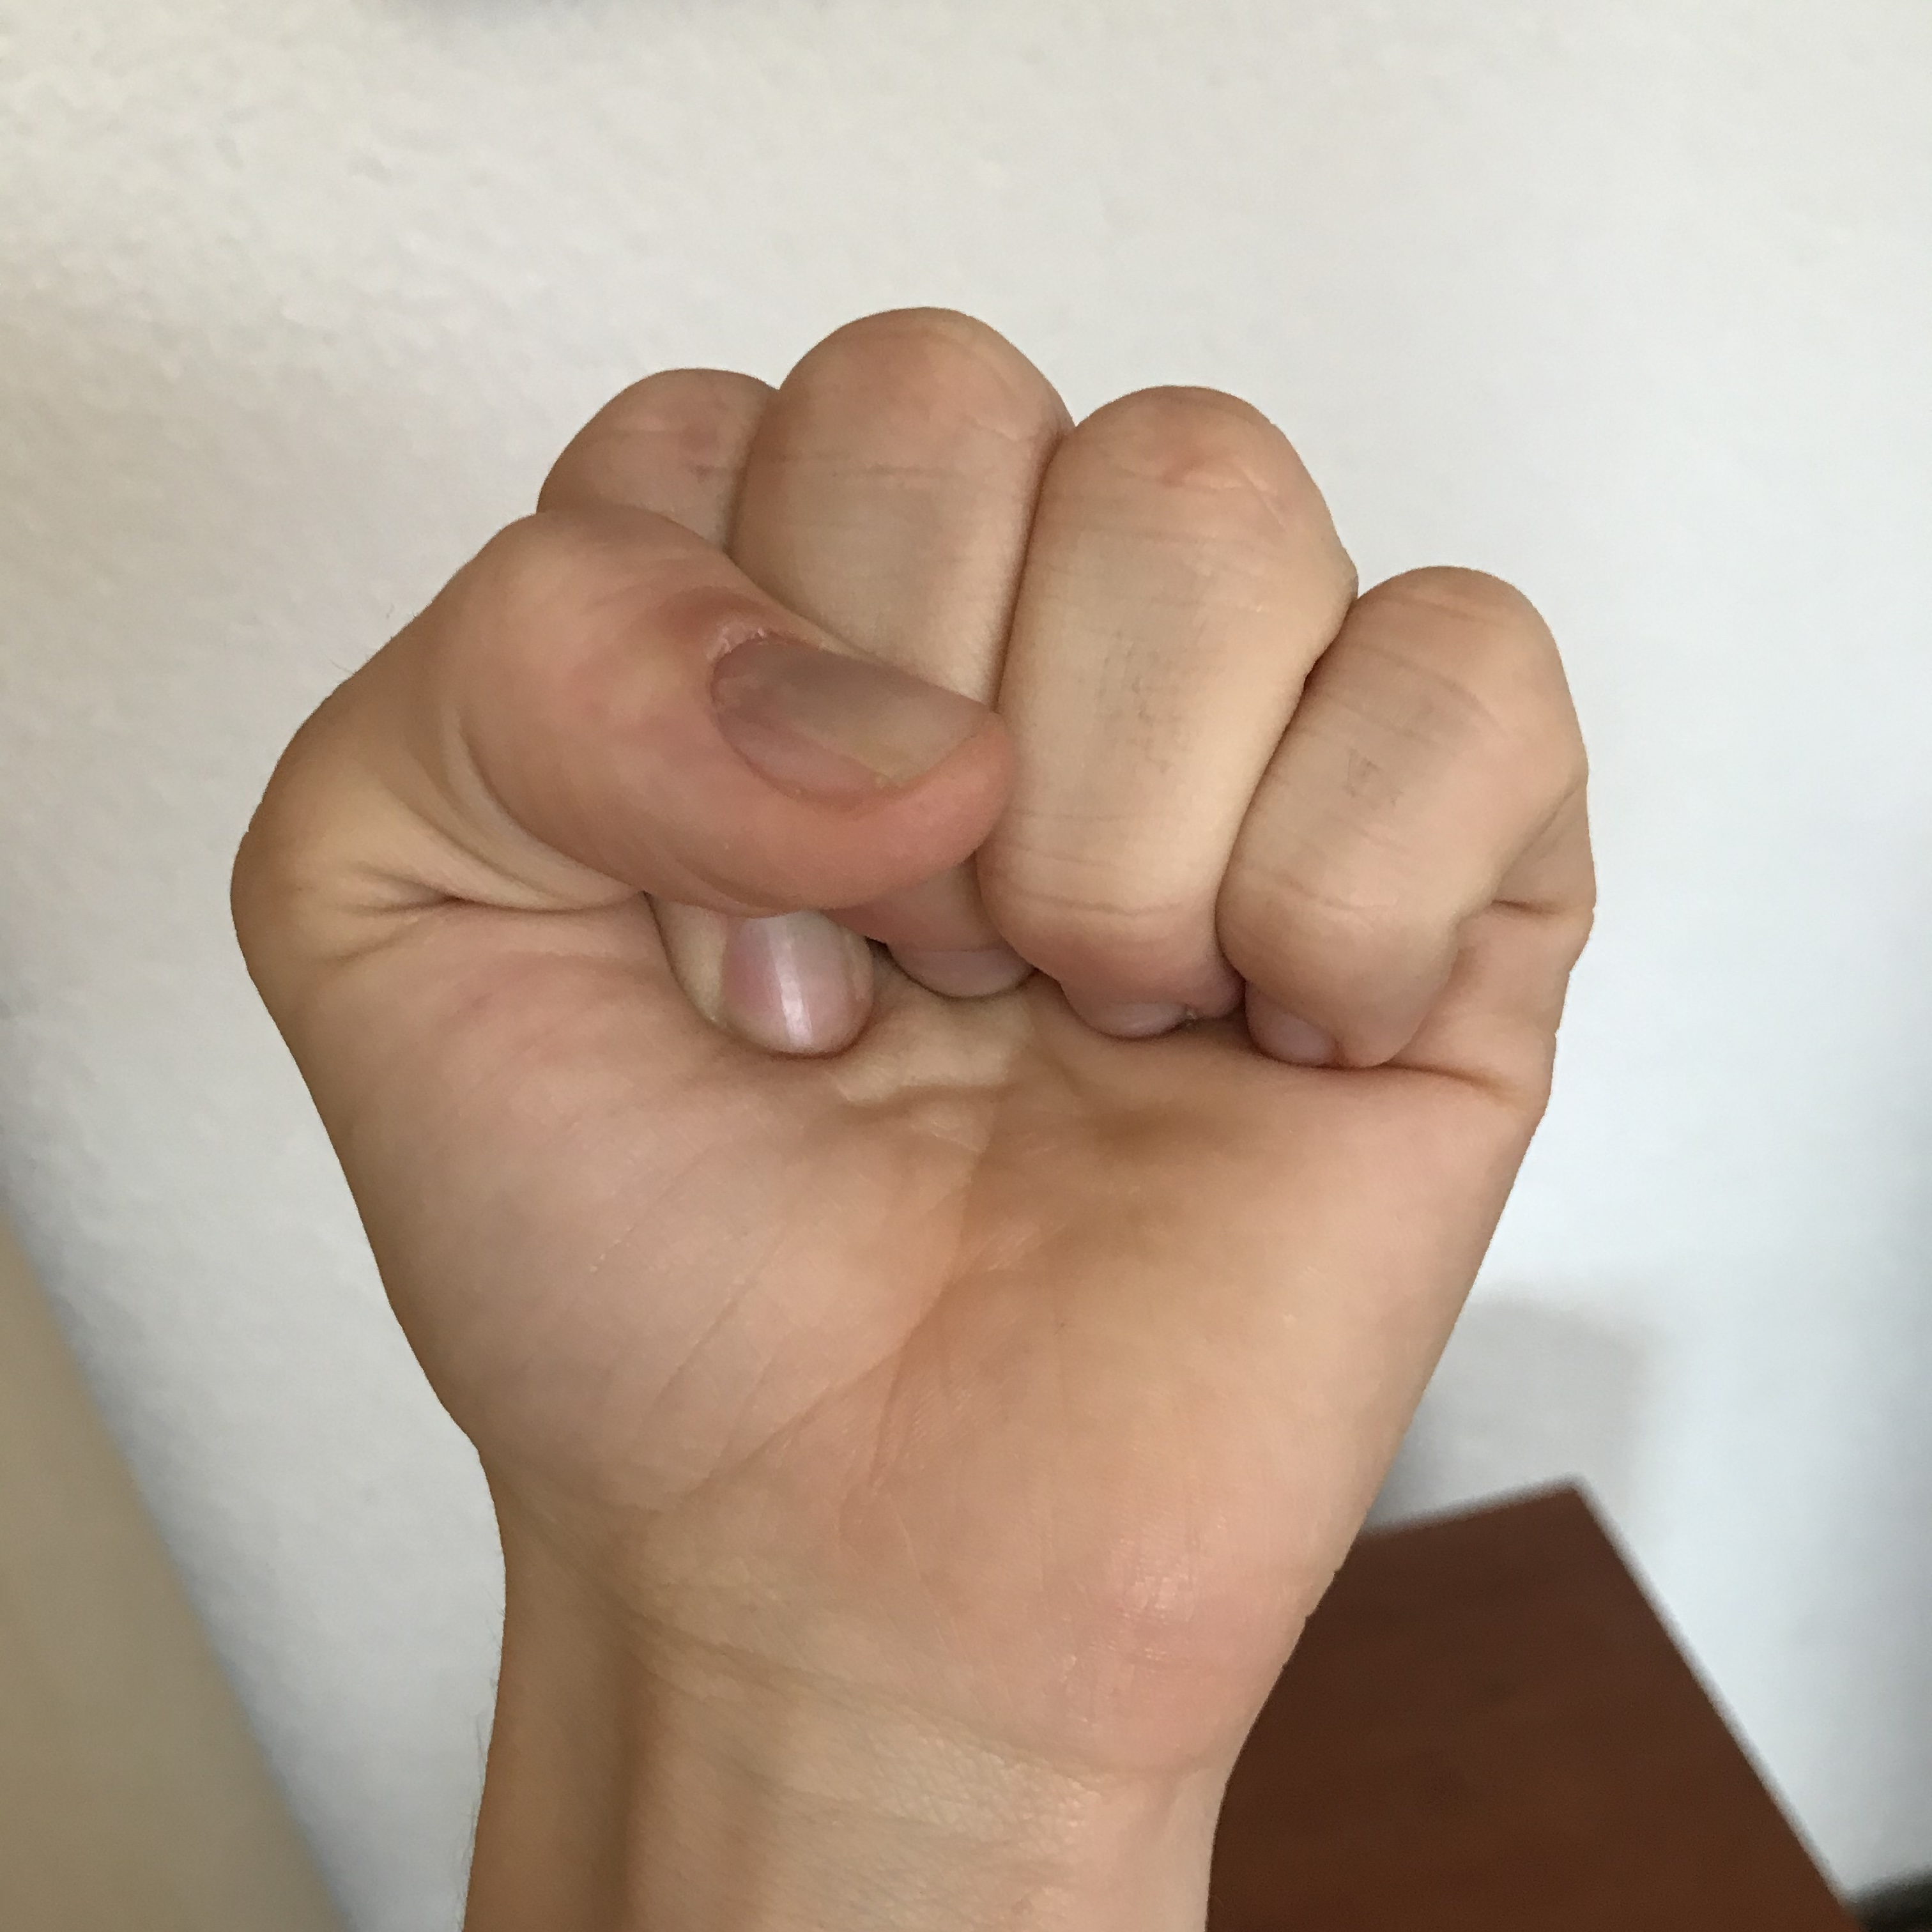
\includegraphics[width=\textwidth]{pictures/klarfaust.jpg}
            \caption[]%
            {{\small Klar erkennbare Faust}}    
            \label{fig:klarfaust}
        \end{subfigure}
        \quad
        \begin{subfigure}[b]{0.475\textwidth}   
            \centering 
            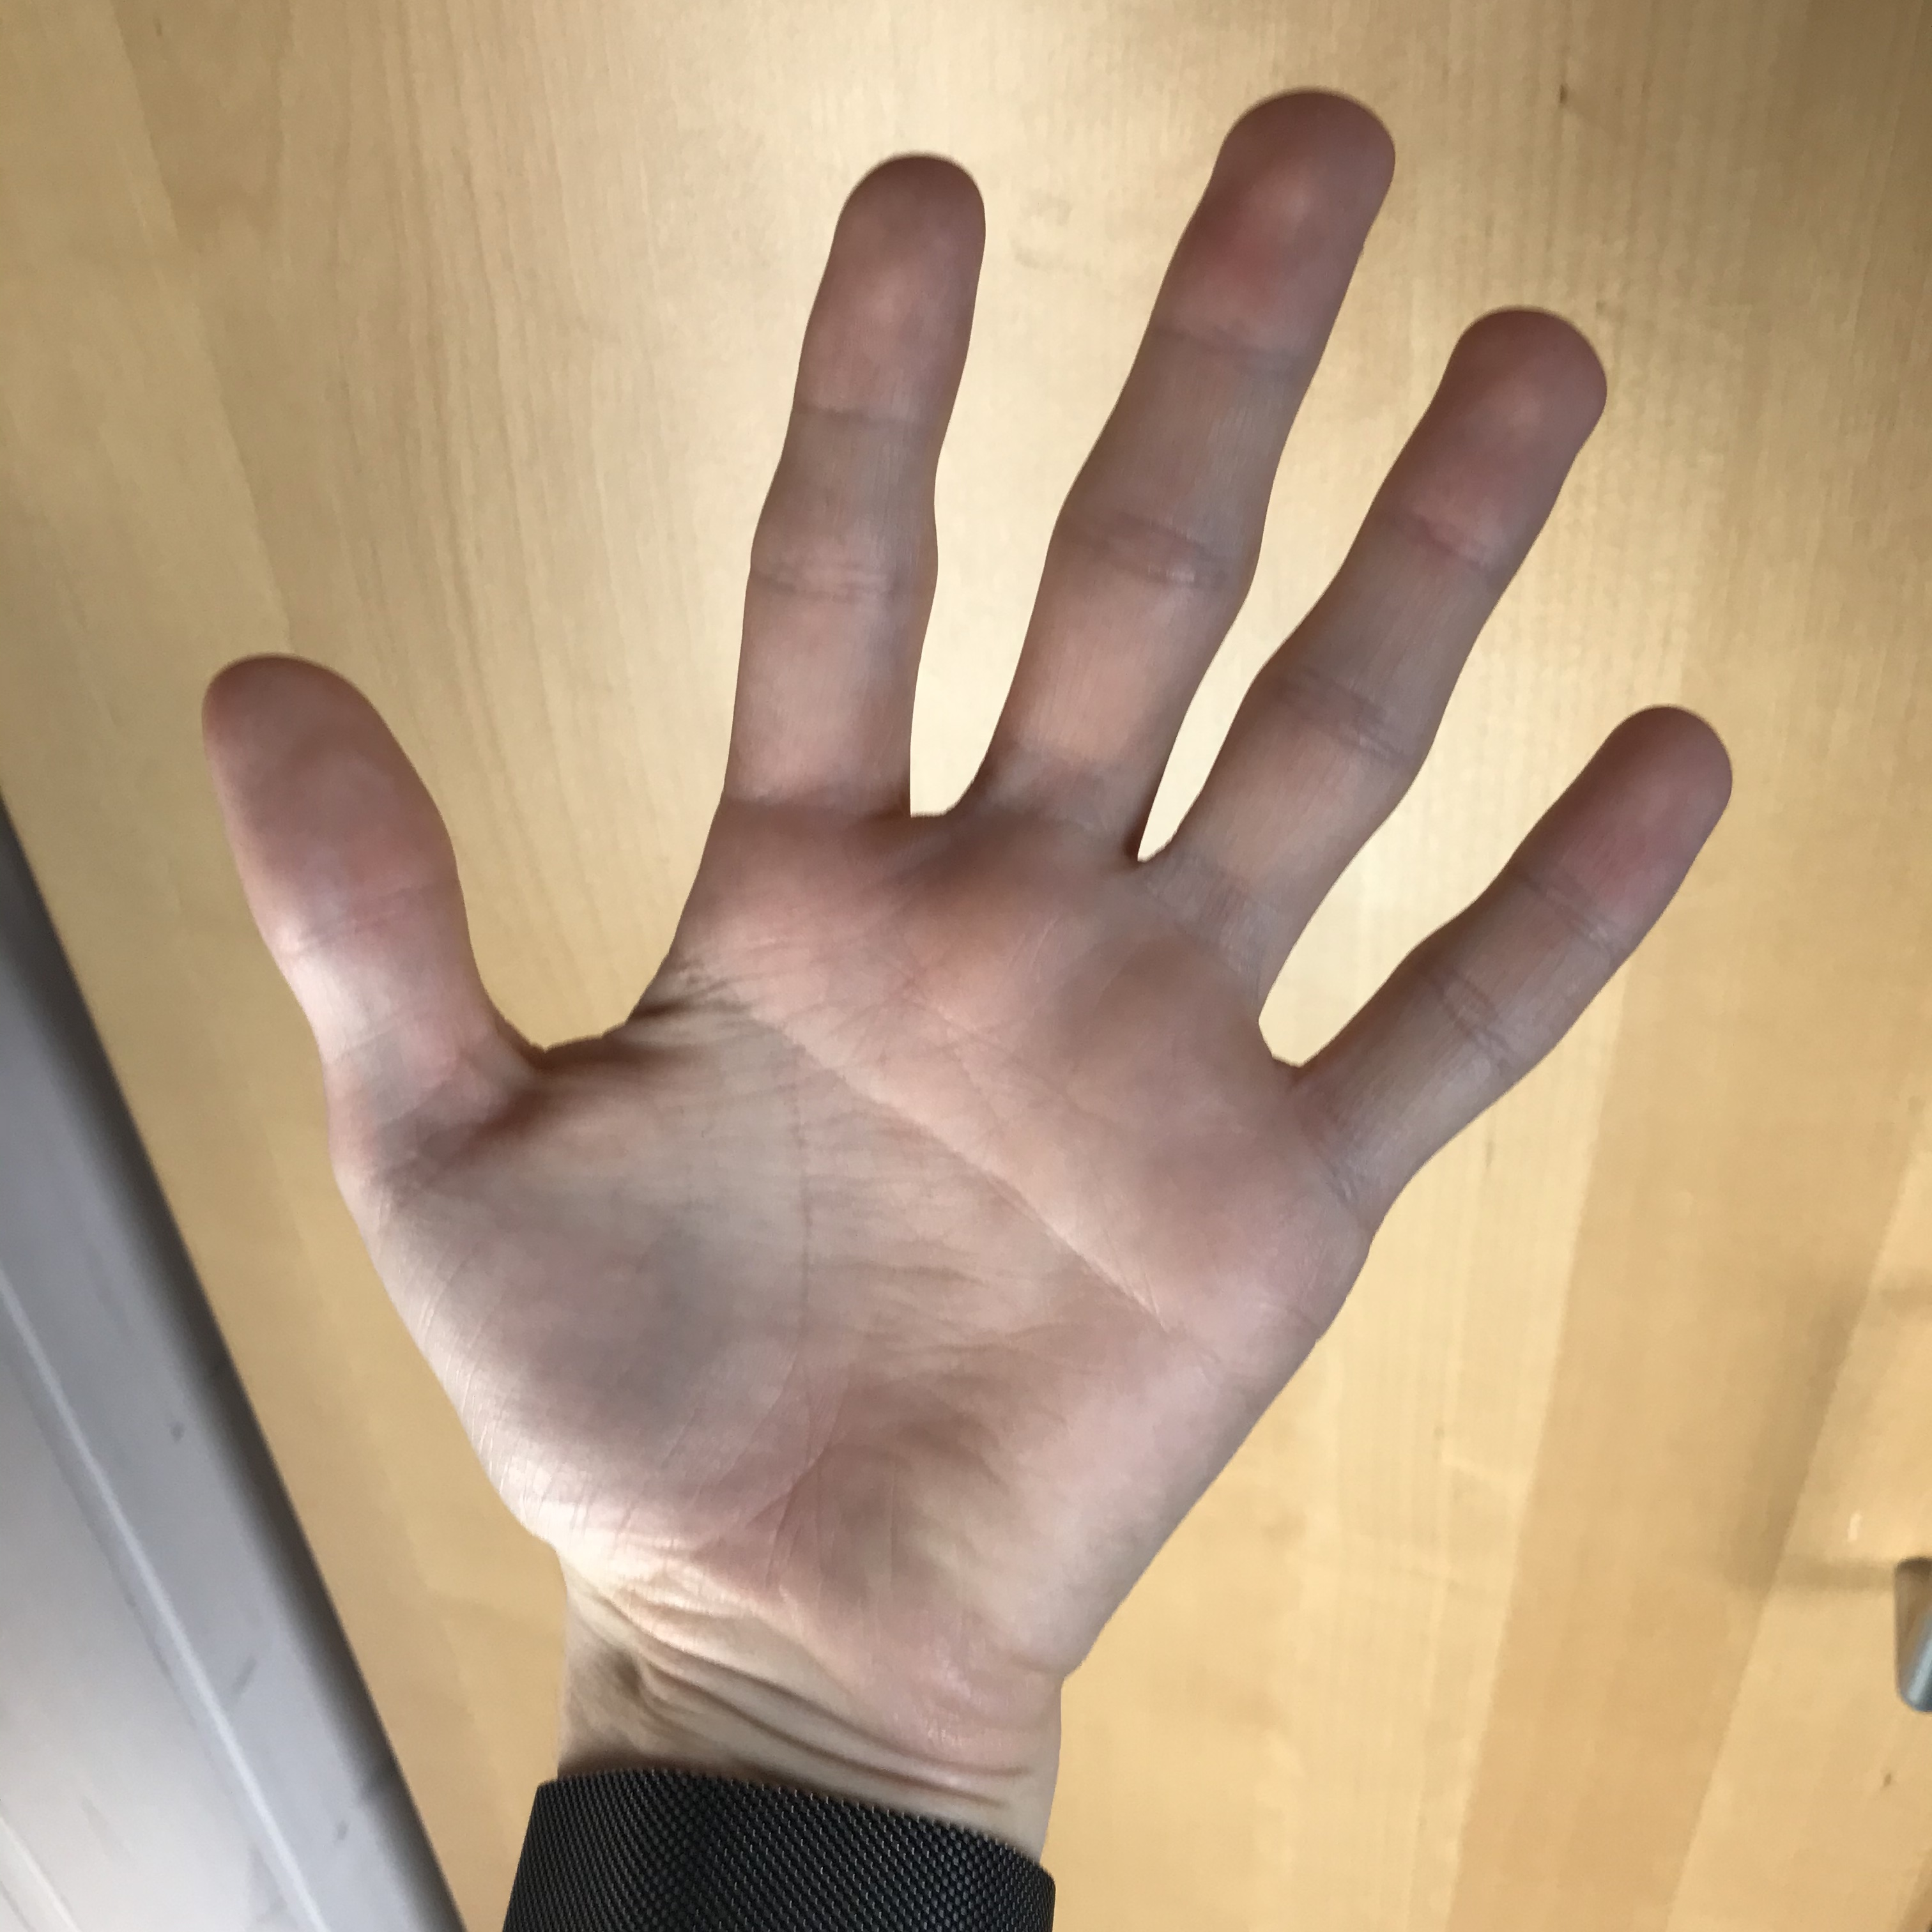
\includegraphics[width=\textwidth]{pictures/klaroffen.jpg}
            \caption[]%
            {{\small Klar erkennbare gespreizte Hand}}    
            \label{fig:klaroffen}
        \end{subfigure}
        \caption[]
        {\small Qualität der Trainingsdaten beeinflusst das Ergebnis der KI.} 
        \label{fig:qualityoftraining}
    \end{figure*}
\newpage
\subsection{Künstliche Intelligenz implementieren}
Die KI zu trainieren ist ein Punkt, aber Sie muss noch mit der App verknüpft werden, dies nennt man das ,,Implementieren``. Die Implementation ist ein langer Prozess mit vielen Details, welche ich hier nur grob dokumentiere. Die Anwendung des erhaltenen ML Model geschieht mithilfe von Vision, ein Framework konzipiert einzig und allein für die Anwendung von Künstlicher Intelligenz. Dies ist ein Prozess aus drei Schritten. Zuerst definiert man einen Request, das ist der erste Teil. Im Request spezifiziert man was man schlussendlich erhalten will und was erkennt werden soll. Der zweite Teil ist der Request Handler, in diesem Teil wird der KI die zu analysierten Daten überbracht. Mit anderen Worten schiesst die Kamera konstant Bilder, welche dann der Künstlichen Intelligenz übertragen und von dieser analysiert werden. Im dritten Schritt werden die Observierungen der Künstlichen Intelligenz ausgewertet und demnach auch Aktionen aufgrund von diesen Beobachtungen ausgeführt. \cite{gesturecontrolvideo}\\ Im letzten Schritt wird auch klar, wieso eine Genauigkeit von 91\% ausreichend ist für eine Gestensteuerung. Verantwortlich ist dieser Stück des Codes: 
\begin{lstlisting}[language=Swift,caption={KI Buffer},label={lst:buffer}]
let bufferSize = 5
var commandBuffer = [RemoteCommand]()
var currentCommand:RemoteCommand = .none{
    didSet {
        commandBuffer.append(currentCommand)
        if commandBuffer.count == bufferSize {
            if commandBuffer.filter({$0 == currentCommand}).count == bufferSize{
                showAndSendCommand(currentCommand)
            }
            commandBuffer.removeAll()
        }
    }
}
\end{lstlisting}
Hier wird ein Buffer erstellt. Die Variable ,,currentCommand`` wird mit jedem Bild und der neuen Schätzung der KI aktualisiert, dies 24 mal in der Sekunde. Wenn man diese Variable mit jedem Bild ausgibt. Dann die Faust macht sie wieder öffnet und dann die Hand wegnimmt, bekommt man eine solche Stringfolge:
\begin{lstlisting}[caption={Output KI-Resultate},label={lst:outputKI}]
Fist, Fist, Fist, Fist, Fist, Fist, Fist, Fist, Fist, Fist, Fist, Fist, Fist, Fist, Open, Open, Open, Open, Open, Open, Open, Open, Open, Open, Open, Open, Open, Open, Open, Open, Open, Open, Open, Open, Open, Fist, Fist, Nothing, Nothing, Nothing, Nothing, Nothing, Nothing, Nothing, Nothing, Nothing, Nothing, Nothing
\end{lstlisting}
Der Buffer geht jedes Element durch und schaut nun wo fünf gleiche Elemente hintereinander folgen, falls dieser Fall eintritt wird die Aktion ausgeführt. Dies schliesst Fehlentscheidungen aus. Dadurch wird die Wahrscheinlichkeit bei einer Genauigkeit von 91\% für eine Fehlentscheidung von 9\%  auf 0.0006\% reduziert.\\Dies wird mithilfe dieser Wahrscheinlichkeitsrechnung berechnet:
\[100\%*0.09^{5} = 0.00059049\%\]
Diese Berechnung basiert allerdings auf den Testresultaten und ist stark abhängig von den Testdaten, sollte also nicht zu ernst genommen werden. Man kann so folgern, dass es sehr selten zu einer Fehlentscheidung im getesteten Situationen kommen soll. Ein Nebeneffekt des Buffers ist eine kleine Verzögerung. Die Gestensteuerung funktioniert besser als erwartet, sogar in dunklen Räumen oder mit verschiedenen Handtypen funktioniert sie sehr gut. Einzig mit besonders grossen Händen hatte die KI Schwierigkeiten und bei falschem Abstand.

\subsection{Publikation auf dem App Store}
Sobald die App fertig ist fehlt nur noch die Publikation. Da meine App in der Programmierumgebung Xcode mit Swift programmiert wurde ist nur eine Veröffentlichung auf dem App Store möglich. Die Publikation setzt mehrere Punkte voraus. Allererstes benötigt man einen Apple Developer Account, welcher 100 CHF im Jahr kostet. Mit diesem kann man so viele Apps wie man will veröffentlichen. Diese muss man bereitstellen um Apps zu auf dem App Store zu veröffentlichen. Auch sollte die App natürlich gegen keine Richtlinien von Apple verstossen, sowie deren Designgrundlagen folgen. Mit diesem Punkt will Apple vor allem Designfehler vorbeugen, also falls sich gewisse Designelemente überlagern oder schlecht angeordnet sind kriegt man bei diesem Punkt Probleme. Ebenfalls braucht man eine Website mit einer ,,Privacy Policy``, dies ist eine Website mit Bestimmungen für Behandlung von Nutzerdaten. Eine solche Website lässt sich über Drittanbieter, wie Flycricket, kostenlos generieren mit allen wichtigen rechtlichen Bestimmungen die man braucht. Dieser Punkt war bei meiner App relativ unbedenklich, da die App lediglich die Kamera benötigt und jegliche Informationen lokal ausgewertet werden, sowie Rezepte und Bilder lokal gespeichert sind. Die Publikation setzt auch eine Entwicklerwebsite voraus, ebenfalls lässt sich diese in Flycricket umsetzten. Ein App-Icon wird genauso benötigt wie mindestens ein Screenshot und eine Beschreibung der App. Screenshots sind nicht immer nur Bildschirmfotos, vielmehr ist dies heutzutage ein Bildschirmfoto in einem Bild eines Smartphones mit Text und Hintergrund (siehe Abb. \ref{fig:Screenshot}). Solche Screenshots lassen sich ebenfalls über Flycricket erstellen. Als Icon (siehe Abb. \ref{fig:logo}) verwendete ich den Buchstabe G mit einem darin versteckten C, welche die Initialen von GestureCook darstellt. 
\begin{figure}
	\centering
	\begin{subfigure}[b]{0.3\linewidth}
    		
\includegraphics[width=\linewidth]{pictures/GestureCookLogo.png}
    		\caption{GestureCook Logo}
    		\label{fig:logo}
    \end{subfigure}
    \begin{subfigure}[b]{0.5\linewidth}
    		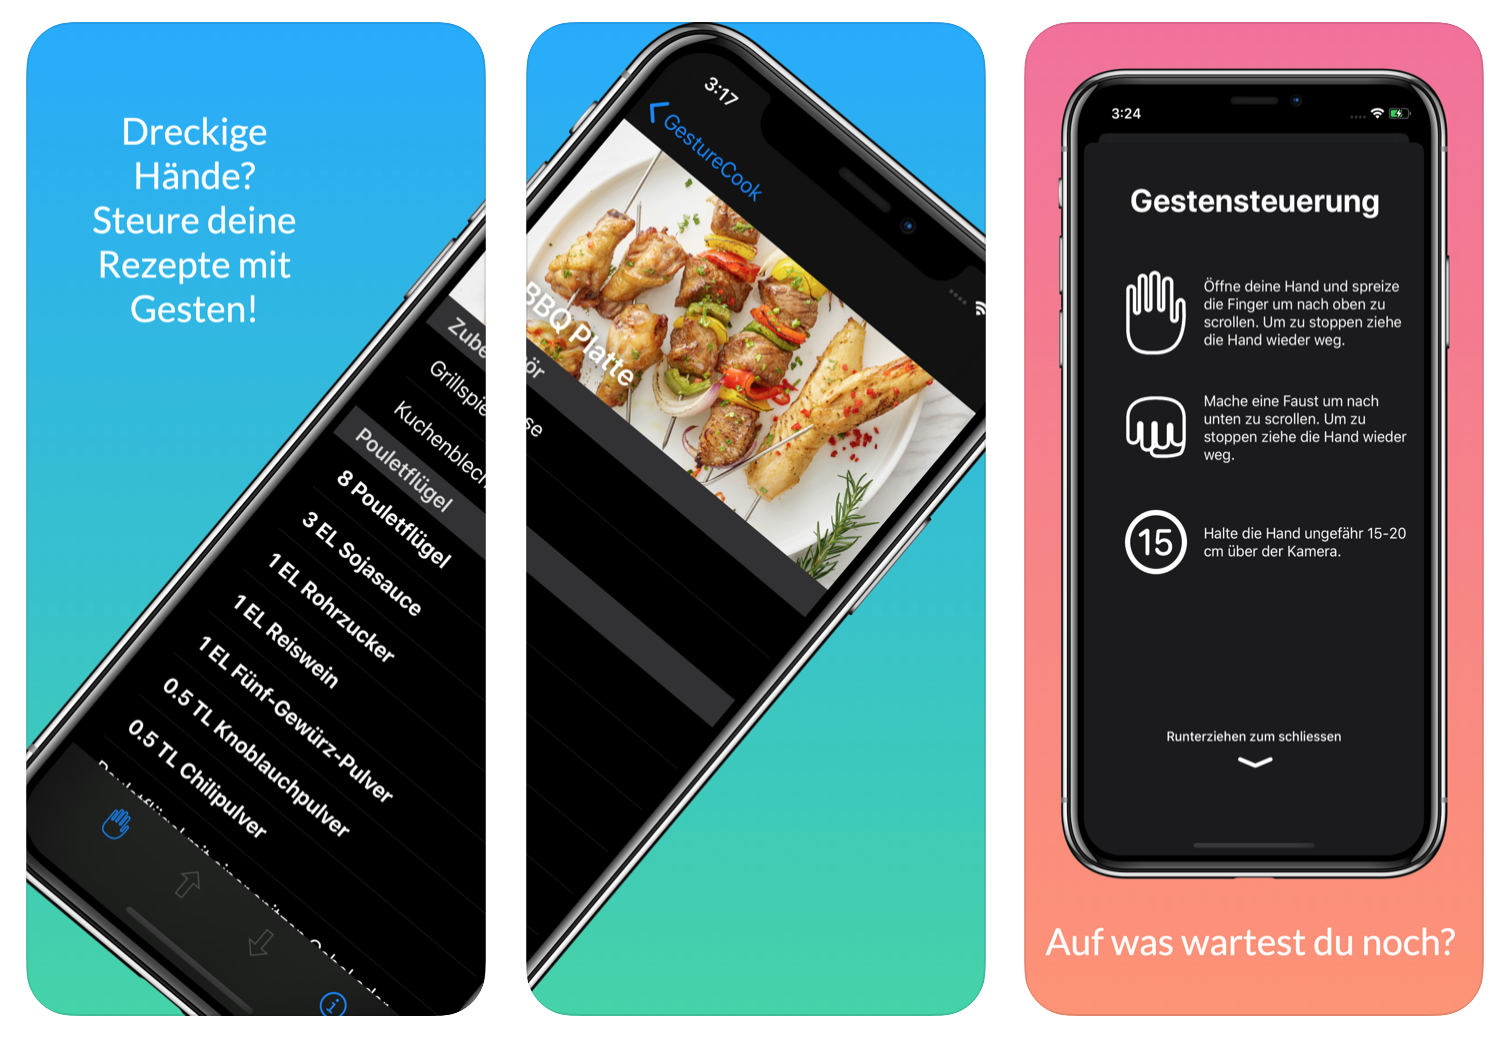
\includegraphics[width=\linewidth]{pictures/Screenshot.png}
    		\caption{GestureCook Screenshots}
    		\label{fig:Screenshot}
    \end{subfigure}
    \caption{Grafische Elemente einer einer AppStore Publikation}
\end{figure}
Schlussendlich sendet man die App ein und man wird entweder angenommen oder abgelehnt und muss die App überarbeiten. Bei mir ging dies allerdings ohne Probleme und wurde beim ersten Versuch angenommen. Die App ist nun im App Store verfügbar und momentan kostenlos erhältlich.
\section{Fazit}
Das Projekt hatte eine breite Themenspanne, ich lernte eine KI anzuwenden, zu trainieren, Tabellen mit spezifisch abgestimmten Zellen zu erstellen und natürlich den XML-Parser zu kodieren. Insgesamt hatte ich wenig Probleme, mit der Ausnahme von falsch ausgewählten Gesten und tiefer Qualität des Datenmaterials. Also müssen bei einer Gestensteuerung die Gesten klar erkennbar sein. Demnach müssen die Trainingsdaten von hoher Qualität sein, denn auch grosse Bildermengen können schlechte Daten schwer ausgleichen. \\ Das Projekt zeigt, dass es nicht  so schwer ist eine Künstliche Intelligenz zu verwenden. Dies ist der Fall, weil bestehende Libraries einem helfen, mit wenig Aufwand gute Resultate zu erreichen. Es ist nach meiner Einschätzung schwerer einen XML-Parser in Xcode zu erstellen, denn je nach XML-Datei sieht dieser wieder anders aus und muss auf den Anwendungsbereich angepasst werden. Die Gestensteuerung funktioniert einiges besser als erwartet und erkennt die Gesten in fast allen Umgebungen. Sie lässt einem auch mit dreckigen Händen die App bedienen. Mit einem Buffer lässt sich die Wahrscheinlichkeit für eine Fehlentscheidung noch um ein Vielfaches verkleinern, hinterlässt allerdings eine kleine Verzögerung. Im Ganzen war dieses Projekt ein Erfolg und ich bin positiv Überrascht vom Ergebnis.

\bibliographystyle{unsrt}
\renewcommand\refname{Bibliografie}
\newpage
\bibliography{main}

\end{document}